\documentclass[11pt]{article}
\usepackage{amsmath,amsthm,amssymb,fullpage,graphicx,hyperref,listings}
\usepackage{listings,color,setspace}
\author{Andy Reagan}
\title{Math 337 Homework 17}

     \def\NN{\mathbb{N} }
     \def\ZZ{\mathbb{Z} }
     \def\QQ{\mathbb{Q} }
     \def\RR{\mathbb{R} }
     \def\CC{\mathbb{C} }
     \def\f{\frac }
     \def\b{\begin }
     \def\e{\end }
     \def\Log{\text{Log} \,}
     \def\Re{\text{Re} \, }
     \newcommand{\pdiff}[2]{\frac{\partial #1}{\partial #2}}
     \newcommand{\partialdiff}[2]{\frac{\partial #1}{\partial #2}}
     \newcommand{\pdiffsq}[2]{\frac{\partial^2 #1}{{\partial #2}^2}}
     \newcommand{\pdiffcu}[2]{\frac{\partial^3 #1}{{\partial #2}^3}}
     \newcommand{\pdiffhi}[3]{\frac{\partial^#3 #1}{{\partial #2}^#3}}
     \newcommand{\diff}[2]{\frac{{\rm d}#1}{{\rm d}#2}}
     \newcommand{\diffsq}[2]{\frac{{\rm d}^{2}#1}{{\rm d} {#2}^2}}
     \newcommand{\diffhi}[3]{\frac{{\rm d}^#3 #1}{{\rm d} {#2}^#3}}
     \newcommand{\tdiff}[2]{\mbox{d} #1/\mbox{d} #2}
     \newcommand{\tdiffsq}[2]{\mbox{d}^{2} #1/\mbox{d} {#2}^2}
     \newcommand{\tpdiff}[2]{\partial #1/\partial #2}
     \newcommand{\tpdiffsq}[2]{\partial^2 #1/\partial {#2}^2}
     \newcommand{\bvec}[1]{\vec{ {\bf #1 } }}
     \newcommand{\oh}[1]{O(h^{{#1}})}

\lstset{language=MATLAB,
basicstyle=\ttfamily\scriptsize\singlespacing,
keywordstyle=\color{black},
stringstyle=\color{black},
commentstyle=\color{black},
morecomment=[l][\color{black}]{\#},
frame=L,
xleftmargin=\parindent,
%%numbers=left,                   %% where to put the line-numbers
%%numberstyle=\scriptsize,      %% the size of the fonts that are used for the line-numbers
%%stepnumber=1,                   %% the step between two line-numbers. If it is 1 each line will be numbered
numbersep=5pt,
breaklines=true,        %% sets automatic line breaking
breakatwhitespace=false,    %% sets if automatic breaks should only happen at whitespace
escapeinside={\%*}{*)} 
}

%% example code insert
%% \lstinputlisting[language=Matlab]{andy_hw12_prb01.m}

%% example figure
%% \begin{figure}[h!]
%%   \centering
%%     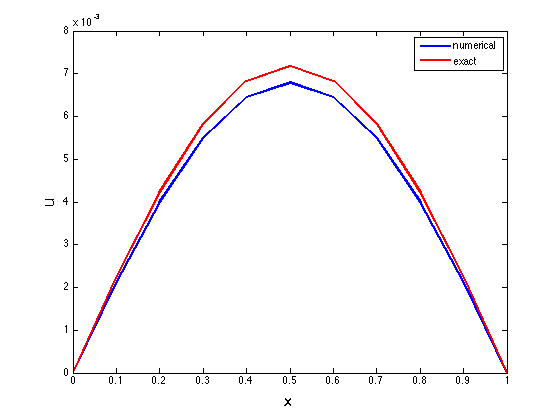
\includegraphics[width=0.45\textwidth]{andy_hw12_prb01_02.png}
%%   \caption{The numerical and exact solution for $h=0.1$.}
%% \end{figure}

%% start problem on next page
%% \clearpage
%% \pagebreak

\begin{document}
\maketitle

\begin{enumerate}

\item We solve using the method from the notes.

What we observe is a shock that moves to the right.
This movement is expected since the initial disturbance is positive, and therefore the characteristic is like $x-ct$ with $c$ positive.
The solution becomes multi-valued for $t>t^*$, where $t*$ is somewhere just greater than 1/4, from our plot.
This is not a phycially plausible situation, and as such our mathematical model has broken down.
A physical analogy would be a piston pushing down on a pipe: here the piston moved too rapidly for the gas to be simply compressed, and the gas has formed a shock wave.
This manifests itself as a discontinuity, which our equation does not model.
%% example code insert
\lstinputlisting[language=Matlab]{andy_hw17.m}

%% example figure
\begin{figure}[h!]
  \centering
    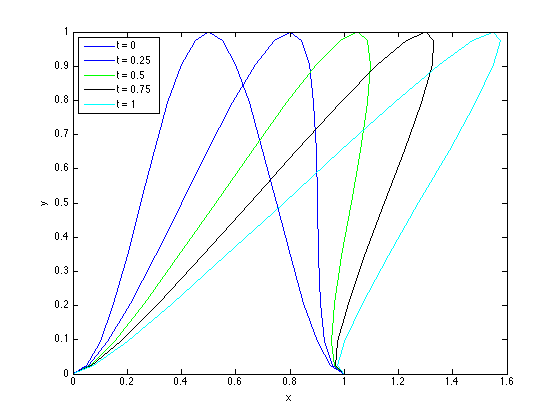
\includegraphics[width=0.85\textwidth]{andy_hw17_01.png}
  \caption{Solution plotted for the specified times.}
\end{figure}

\end{enumerate}
\end{document}



